\newcommand{\mcG}{\mathcal{G}}
\newcommand{\mcV}{\mathcal{V}}
\newcommand{\mcE}{\mathcal{E}}
\newcommand{\bfitx}{\symbfit{x}}

\chapter{Basics of Geometric Deep Learning and Graph Neural Networks}\label{chap:gnn}

\section{Graphs}\label{sec:graphs}

In various branches of science, from biology to particle physics, graphs are often used as models of systems of relations and interactions. In this work, graphs are important as they engender a fundamental type of permutation invariance.

A basic \textbf{graph} \(\mcG=\left(\mcV, \mcE \right)\) is a collection of \textbf{nodes} $\mcV$ and \textbf{edges} \(\mcE\subseteq \mcV \times \mcV\) between pairs of nodes. Depending on the application or field, the nodes can also be called \textbf{vertices}, and the edges can be called \textbf{links} or \textbf{relations}.

For the purpose of an intuitive explanation, we assume that the nodes are associated with $s$-dimensional \textit{node features}, denoted by $\symbfit{x}_u$ for all $u \in \mcV$. Social networks are one of the most studied and best examples of graphs in the real world. Here, nodes represent users, edges correspond to friendship relations between them, and node features ($\symbfit{x}_u \in \mathbb{R}^d$) model user information such as age, location, last active time, etc. It should be noted that it is often possible to equip edges with features.
%however, this is not of concern within the scope of this work. Please refer to the detailed geometric deep learning text by \textcite{Bronstein2021}.


\begin{wrapfigure}{r}{0.25\textwidth}
    \centering
    % \captionsetup{justification=RaggedRight}
    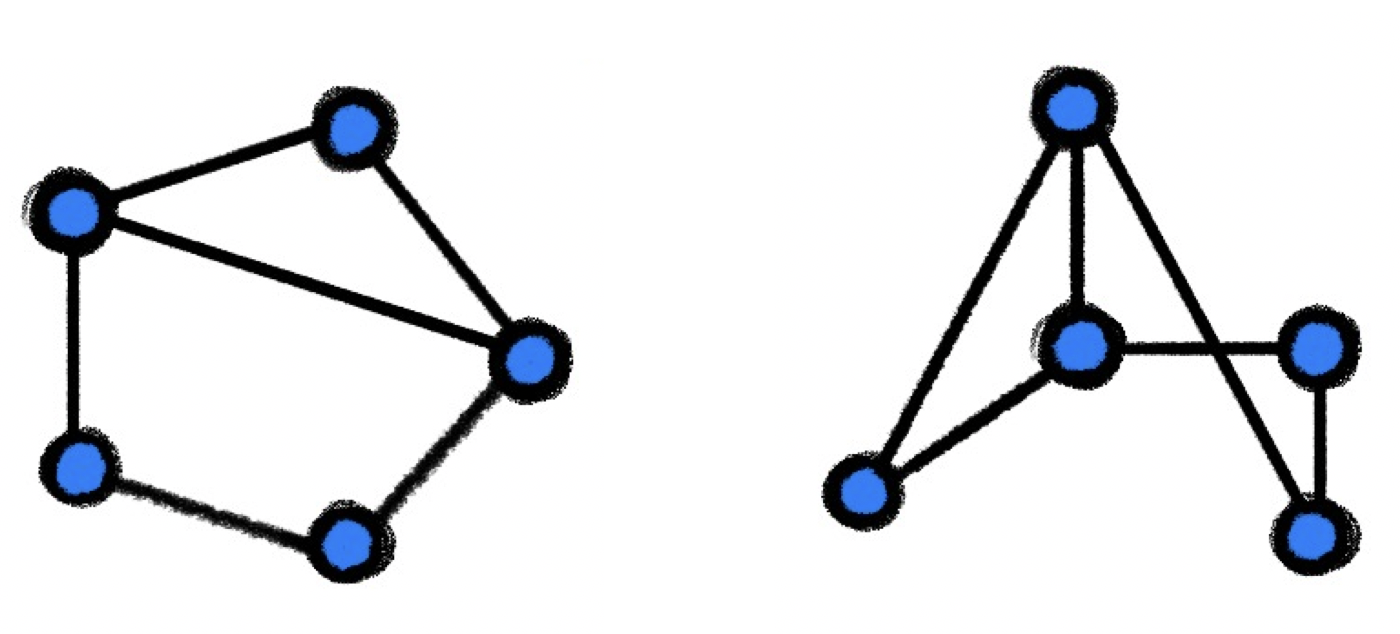
\includegraphics[scale=0.15]{chapters/assets/graph-figs/mn_isomorphic.png}
    \caption{Two isomorphic graphs}
    \label{fig:graph-isomorphism}
\end{wrapfigure}
A key property of graphs is that nodes in $\mcV$ are not typically assumed to be provided in any particular ordering, and thus, by extension, any operations performed on graph structures should not depend on any assumed inherent ordering of nodes. The desirable property that functions acting on graphs must possess is called \textbf{permutation invariance}, and implies that for any two \textbf{isomorphic} graphs, the results of such functions must be identical. {\em Isomorphism} is an edge-preserving bijection between two graphs. The two isomorphic graphs shown in \cref{fig:graph-isomorphism} are identical up to the reordering of their nodes.

Permutation invariance is important in \highlight[comment=add ref to article]{\samptr.} One of the main motivations behind \samptr\ is to allow the network to learn from multiple samples made available to the network in the form of a mini-batch. The ordering of the samples is of little interest to us as we are more concerned with learning by looking beyond single instances. The exact mechanism of this will be explained in more detail in subsequent sections.



\section{Janossy Pooling}
Let us first illustrate the concept of permutation invariance on \textbf{sets}, a special case of graphs without edges ($\mcE=\emptyset$). We illustrate this with the help of a framework provided to us in the form of Janossy pooling \parencite{Murphy2018}.

Currently, there are a few ways to incorporate permutation invariance. The first is the ``permute and average'' paradigm. It works by considering all possible permutations of input elements, then passing each permutation through a permutation-sensitive model or function, and then taking an average of all the results. If two inputs $\symbf{X}$ and $\Tilde{\symbf{X}}$ are permutations of each other, this process will give the same result for both inputs. Mathematically, this can be written as follows:
\begin{equation}
    \label{eqn:perm-invar-avg}
    \widehat{f}(\symbf{X}) = \frac{1}{|{T}_n|} \sum_{\pi \in {T}_n} \phi \bigl( \pi \left( \symbf{X} \right) \bigr)
\end{equation}
where $\symbf{X}=\left(\symbfit{x}_1, \ldots, \symbfit{x}_n\right)^\top$ is a stack of node features and has $n$ elements with $d$ dimensionality, $T_n$ is the set of all permutations of $n$ elements, and $\phi$ is a permutation-sensitive model. Therefore, we construct a permutation-invariant $\widehat{f}$ from a permutation-sensitive $\phi$.

This idea is called \textbf{Janossy pooling} and was first introduced by \textcite{Murphy2018}. Indeed, it is a straightforward and easy way to achieve permutation invariance, but it happens to be very computationally intensive. The computational cost is dominated by the sum over $T_n$ in \cref{eqn:perm-invar-avg}, where the number of elements in $T_n$ is $n!$. As one can imagine, if $\symbf{X}$ is a mini-batch with very large $n$, \cref{eqn:perm-invar-avg} quickly becomes intractable.

\begin{figure}[bh]
    \centering
    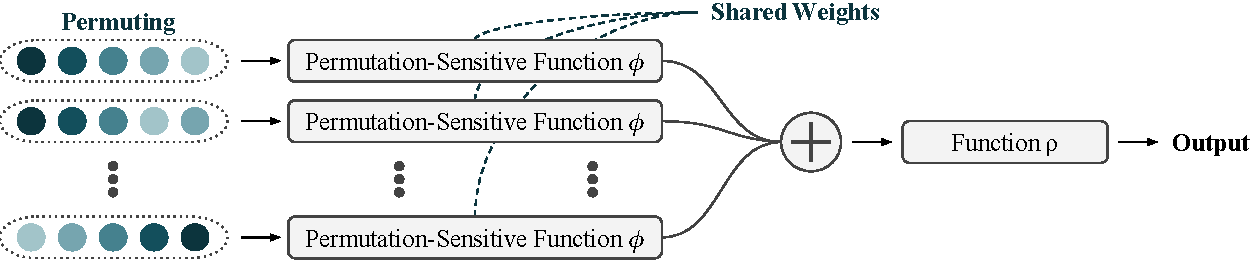
\includegraphics[width=\textwidth]{chapters/assets/graph-figs/permuting.pdf}
    \caption{$\widehat{f}$ comprises everything up to and including the sum. The function $\rho$ coming after the sum is optional and does not need to follow any constraints to guarantee invariance because its input, $\widehat{f}(x)$, is already invariant. Image courtesy of borrowed from \textcite{wagstaff2022universal}.}
    \label{fig:basic-perm-invar}
\end{figure}
\footnotetext{\url{https://fabianfuchsml.github.io/learningonsets}}

\subsection{A More Efficient Janossy Pooling}\label{ssec:efficient-janossy}

To save computational costs, we may give up the calculation of $n!$ permutations. In the above (\Cref{fig:basic-perm-invar}), we look at all possible $n$-tuples from the set of $n$ elements; instead, we can consider all $k$-tuples where $k \less n$ \parencite{Murphy2018}. We can then update \cref{eqn:perm-invar-avg} as:
\begin{equation}
    \label{eqn:k-tup-janossy}
    \widehat{f}(\symbf{X}) = \frac{1}{|P(n, k)|} \sum_{\symbf{X}_{\{k\}}} f(\symbf{X}_{\{k\}})
\end{equation}
where $\symbf{X}_{\{k\}}$ stands for a $k$-tuple of $\symbf{X}$.

Let us take a short example to understand how the count of values came about in \cref{eqn:k-tup-janossy}. Consider the input set ${w, x, y, z}$ with $n=4$. When we set $k=2$, then our sum will be applied over all $2$-tuples:
\[(w, x),~(x, w),(w, y),~(y, w),~(w, z),~(z, w),
(x, y),~(y, x),~(x, z),~(z, x),~(y, z),~(z, y)
\]
A sum over all these tuples is clearly invariant to permutations of elements in the input set, that is, each tuple appears exactly once in the sum no matter the order of individual elements. Therefore, the number of $k$-tuples from a set of $n$ elements is:
\begin{equation}
\label{eqn:k-tup-cnt}
    P(n,k) = \frac{n!}{(n-k)!}
\end{equation}

For $k \ll n$, this gives us a much more tractable method. Setting $k=n$ gives us the most expressive and most expensive model. Setting $k=1$ gives us a model whose cost is linear in the size of the input set. Increasing $k$ allows us to take into account higher-order interactions between elements in the set; we will come back to this idea of interactions in \Cref{ssec:relation-and-interactions}.

\begin{figure}[th]
    % \vspace{-0.2cm}
	\centering
% 	\hspace{-1cm}
	\begin{subfigure}[h]{0.46\textwidth}
		\centering
		\captionsetup{justification=centering}
		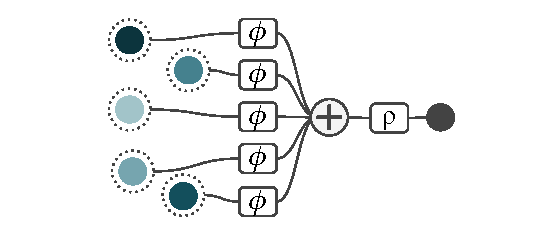
\includegraphics[width=0.99\textwidth]{chapters/assets/graph-figs/Janossy_K1.pdf}
		\caption{Janossy pooling with $k=1$ (\emph{Deep Sets})}
		\label{fig:Janossy_K1}
	\end{subfigure} 
	\begin{subfigure}[h]{0.46\textwidth}
		\centering
		\captionsetup{justification=centering}
		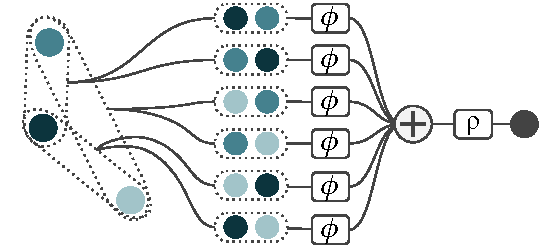
\includegraphics[width=0.99\textwidth]{chapters/assets/graph-figs/Janossy_K2.pdf}
		\caption{Janossy pooling with $k=2$}
		\label{fig:Janossy_K2}
	\end{subfigure} 
	\begin{subfigure}[h]{0.46\textwidth}
	    \vspace{+1cm}
		\centering
		\captionsetup{justification=centering}
		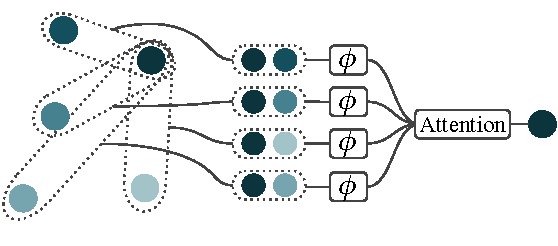
\includegraphics[width=0.99\textwidth]{chapters/assets/graph-figs/Janossy_K2Att.pdf}
		\vspace{-0.8cm}
		\caption{Self-attention}
		\label{fig:Janossy_K2Att}
	\end{subfigure} 
	\caption{Different variations of Janossy pooling. Permutation invariance is guaranteed by processing all combinations of $k$ elements and then aggregating via a sum (or softmax in the case of attention). Self-attention, a variant of Janossy pooling with $k=2$, focuses on one node at a time (the darkest node here), computing an output for this specific node. It is often employed for all nodes in parallel in a permutation-equivariant manner, mapping sets of points to sets of points \parencite{Lee2018}. Image borrowed from \textcite{wagstaff2022universal}.}
	\label{fig:k12}
\end{figure}

\subsection{Deep Sets}\label{ssec:deep-sets}

When $k=1$ and we include the optional function $\rho$, we obtain a popular special case known as Deep Sets \parencite{zaheer2017deep}. \citeauthor{zaheer2017deep} propose a neural architecture in which each input is first transformed by a neural network model $\phi$ individually (see \Cref{fig:Janossy_K1}), then the results are aggregated via a $\operatorname{sum}$ operator and further processed by a second neural network $\rho$.

The aforementioned functions produce a \textquote{global} graph-wise result, but we are frequently more interested in functions that work \textquote{locally} or node-wise. In order to acquire the collection of latent node features, for instance, we would wish to use some function to \textit{update} the features in each node. In other words, we may wish for a \textbf{node-wise} function to be permutation equivariant and want a permutation invariant \textbf{graph-wise} function.

We can now generalise the notions of permutation-invariance and equivariance from sets to graphs. In the generic setting $\mcE \neq \emptyset$, the graph connectivity can be represented by a $n \times n$ \textbf{adjacency matrix} $\symbf{A}$, defined as
\begin{equation}
    \label{eqn:adj-matrix-def}
    a_{u v}= \begin{cases}1 & (u, v) \in \mcE \\ 0 & \text { otherwise }.\end{cases}
\end{equation}

Note that now the adjacency and input (or feature) matrices $\symbf{A}$ and $\symbf{X}$ are \textquote{synchronised}, $a_{u, v}$
specifies the adjacency information between the nodes described by the $u\textsuperscript{th}$ and $v\textsuperscript{th}$
rows of $\symbf{X}$. Therefore, applying a permutation matrix $\symbf{P}$ to node features $\symbf{X}$ directly implies applying it to $\symbf{A}$'s rows and columns, $\symbf{PA}\symbf{P}^\top$. We then say that a graph-wise function $f$ is permutation invariant if 
\begin{equation}
    f\left(\symbf{P X}, \symbf{P A}^{\top}\right)=f(\symbf{X}, \symbf{A})
\end{equation}
and a node-wise function $\phi$ is permutation equivariant if
\begin{equation}
    \phi\left(\symbf{P X}, \symbf{P A P}^{\top}\right)=\symbf{P}\phi(\symbf{X}, \symbf{A})
\end{equation}

\subsection{Modelling Relations and Interactions}\label{ssec:relation-and-interactions}

\samptr\ has yet another fundamental idea that is essential for its success and operation. 
It is able to exploit the interactions (or relations) between elements in a set (mini-batch, which really means that we are trying to capture the fact that our model output may depend not only on the individual contribution of each element, but it may be crucial to also take into account the fact that certain elements appear together in the same set. Our goal is simply to model and use these interactions.

To illustrate this with a simple example, imagine the task of evaluating how well a set of ingredients work together to cook a meal. Setting $k=1$ allows the function $\phi$ to consider related individual attributes, but it cannot detect conflicts between ingredients (e.g., garlic vs. vanilla). Larger $k$ allows $\phi$ to see more than one item at a time, allowing it to make relational inferences about pairs of ingredients, allowing for a more expressive model of deliciousness. Considering $\phi$ as an encoder and $\rho$ as a decoder, $\phi$ can encode information about interactions, which $\rho$ can use for decoding.

Similar to the above example, $\samptr$ uses \highlight[comment=cite/ref here]{contrastive learning} in order to learn to place semantically similar images closer together in an embedding space. When we increase $k$, we give our model the expressivity to learn to recognise semantic similarities between images and to explicitly take these relations into account. By allowing the model to consider relations between images in a mini-batch, it can better decide which images belong closer together in the feature space and in turn learn better discriminative semantic features. Bear in mind that the image is first passed through a CNN (see \Cref{chap:cnn}), and all the other operations explained here are applied to the flattened output of the CNN.

\section{Graph Neural Networks}\label{sec:graph-nn}

Now that we have described graphs 


\section{Janossy Pooling and Self-Attention}\label{sec:jan-attn}

Many of the current neural architectures resemble Janossy pooling with $k=2$.
\textbf{Self-attention} \parencite{vaswani2017attention} is one such algorithm that is also used in the context of graphs in \samptr. Self-attention works by comparing two elements of a set at a time, usually by performing a scalar product.
The results of the scalar products are used as \textbf{attention weights} to aggregate information from different points using a weighted permutation invariant sum. Although it is similar to binary Janossy pooling, self-attention also uses $\operatorname{softmax}$ to ensure that attention weights sum up to $1$ (see \Cref{sec:softmax}).

To substantiate the relationship between permutation-invariant binary Janossy pooling and self-attention, we first define a natural extension of $k$-ary Janossy pooling from permutation \textit{invariance to equivariance}. In normal binary Janossy pooling, the function $\phi$ acts on every two-tuple, followed by the $\operatorname{sum}$-pooling operation. For the purpose of visualisation and intuition, we will write these two-tuples as a matrix:
\[
\begin{bmatrix}
\phi(\bfitx_1, \bfitx_1) & \phi(\bfitx_2, \bfitx_1) & \cdots & \phi(\bfitx_n, \bfitx_1) \\
\phi(\bfitx_1, \bfitx_2) & \phi(\bfitx_2, \bfitx_2) & \cdots & \phi(\bfitx_n, \bfitx_2) \\
\vdots                   &  \vdots              & \ddots & \vdots         \\
\phi(\bfitx_1, \bfitx_n) & \phi(\bfitx_2, \bfitx_n) & \cdots & \phi(\bfitx_n, \bfitx_n)
\end{bmatrix}
\]

If we pool over the \textit{entire matrix} we get an invariant output. However, pooling over \textit{each row individually} we get a permutation equivariant output.
In general we define $k$-ary equivariant Janossy pooling as follows: the $i\textsuperscript{th}$ output is obtained by aggregating overall ($\phi$-transformed) $k$-tuples which start with element $\bfitx_i$. A second network $\rho$ may then further transform each output individually. Mathematically, this reads as:
\begin{equation}
    f_i(\symbf{X}) = \rho \left( \sum_j \phi(\bfitx_i, \bfitx_j) \right)
\end{equation}

In practise, however, the process is slightly more involved. Typically, $\phi(\bfitx_i, \bfitx_j)$ is divided into \textbf{attention weights} $w(\bfitx_i, \bfitx_j)$ and \textbf{values} $v(\bfitx_j)$ and a softmax is applied on the attention weights. Furthermore, the attention weights themselves would be born from the scaled dot-product between two affine transformations called the \textbf{query} and \textbf{key}.
However, the elegant view from the lens of binary Janossy pooling remains clear.